%%%%%%%%%%%%%%%%%%%%%%%%%%%%%%%%%%%%%%%%%%%%%%%%%%%%%%%%%%%%%%%%%%%%%%
%%%%%                                                                %
%%%%%     Document Class                                             %
%%%%%                                                                %
%%%%%%%%%%%%%%%%%%%%%%%%%%%%%%%%%%%%%%%%%%%%%%%%%%%%%%%%%%%%%%%%%%%%%%
\documentclass[%
 halfparskip
]{scrartcl}


%%%%%%%%%%%%%%%%%%%%%%%%%%%%%%%%%%%%%%%%%%%%%%%%%%%%%%%%%%%%%%%%%%%%%%
%%%%%                                                                %
%%%%%     Preamble                                                   %
%%%%%                                                                %
%%%%%%%%%%%%%%%%%%%%%%%%%%%%%%%%%%%%%%%%%%%%%%%%%%%%%%%%%%%%%%%%%%%%%%
\usepackage[utf8]{inputenc}
\usepackage[english]{babel}
\usepackage[T1]{fontenc}

\usepackage{xspace}
\usepackage{graphicx}
\usepackage{amsmath}
\usepackage{amsfonts}
\usepackage{tabularx}
\usepackage{booktabs}
\usepackage{ltxtable}
\usepackage{threeparttable}
\usepackage{pifont}

\usepackage{hyperref}


%% Path to the figures to be used.
\graphicspath{{./figures/}}

%% Do not use sans-serif fonts for all dispositions (chapters,
%% sections, etc.).
\setkomafont{disposition}{\normalfont\bfseries}

%% Do not use sans-serif fonts for the labels of descriptions.
\setkomafont{descriptionlabel}{\normalfont\bfseries}

%% Some custom commands.
\newcommand{\figref}[1]{Figure~\ref{#1}\xspace}
\newcommand{\mmyes}{\checkmark}
\newcommand{\mmno}{$\times$}
\newcommand{\cmark}{\ding{51}}
\newcommand{\xmark}{\ding{55}}

%%%%%%%%%%%%%%%%%%%%%%%%%%%%%%%%%%%%%%%%%%%%%%%%%%%%%%%%%%%%%%%%%%%%%%
%%%%%                                                                %
%%%%%     Document Settings                                          %
%%%%%                                                                %
%%%%%%%%%%%%%%%%%%%%%%%%%%%%%%%%%%%%%%%%%%%%%%%%%%%%%%%%%%%%%%%%%%%%%%
\title{NORX v2.0\\Hardware Architecture}
\author{Michael Muehlberghuber}

% Use the 'hyperref' package in order to set PDF file meta data.
\makeatletter
\hypersetup{
 pdftitle    = {NORX Hardware Architecture},   
 pdfauthor   = {\@author, <mbgh@iis.ee.ethz.ch>},
% pdfkeywords = {<KEYWORDS>},
% pdfsubject  = {<SUBJECT>}
}
\makeatother


%%%%%%%%%%%%%%%%%%%%%%%%%%%%%%%%%%%%%%%%%%%%%%%%%%%%%%%%%%%%%%%%%%%%%%
%%%%%                                                                %
%%%%%     Start of Document                                          %
%%%%%                                                                %
%%%%%%%%%%%%%%%%%%%%%%%%%%%%%%%%%%%%%%%%%%%%%%%%%%%%%%%%%%%%%%%%%%%%%%
\begin{document}

\maketitle

\begin{abstract}
  \textbf{Abstract.} This document contains a brief summary of the
  NORX hardware
  implementation.\footnote{\url{https://github.com/norx/norx-hw}} The
  goal in mind during the development of the architecture was to
  achieve a throughput of 100\,Gbps on a 65\,nm ASIC technology. Our
  architecture solely comprises \mbox{NORX64-4-1}, since this is the
  recommended version of the authors. Version 2.0 of the NORX
  specification was used as a reference for this design.
\end{abstract}


\section{Architecture Overview}

Figure~\ref{lbl:architecture} provides an overview of the developed
NORX64-4-1 hardware architecture. Its major components are the eight
instances of the NORX $G$ function.
%
\begin{figure}[h]
\centering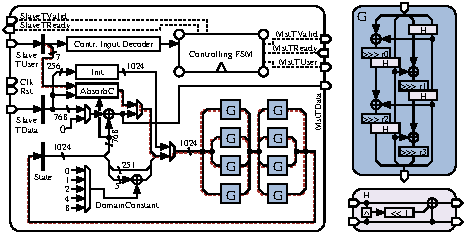
\includegraphics[width=0.85\linewidth]{./figures/norx-arch.pdf}
\caption{NORX64-4-1 architecture overview}
\label{lbl:architecture}
\end{figure}
%
Originally, the architecture was developed for NORX v1.1. For the
submission of the second CAESAR competition round, the authors of NORX
adapted the rate/capacity ratio. Therefore, the hardware architecture
was adapted accordingly.

\section{Features}

The NORX hardware architecture \ldots
\begin{itemize}
\item \ldots supports both encryption and decryption of the
  recommended version of NORX v2.0 (i.e., NORX64-4-1).
\item \ldots takes as input blocks, each of which has the same size as
  the bitrate (i.e., 768\,bits for NORX64-4-1 v2.0).
\item \ldots operates on the byte level, i.e., it can process both
  full as well as non-full input blocks. 
\item \ldots can read inputs and write outputs with the use of two
  AXI-4 Stream Protocols.
\end{itemize}

\section{I/O Interface}

Basically, two AXI4-Stream protocols are used to communicate with the
NORX architecture. For the input data, the \texttt{SlaveTUser\_SI}
signal is used to describe the incoming data (provided via the
\texttt{SlaveTData\_DI} signal). While bits \texttt{14 downto 8} of
the \texttt{SlaveTUser\_SI} signal are used to describe the number of
valid input bytes, the lower eight bits of the \texttt{SlaveTUser\_SI}
signal are used to actually determine what type of input data is
provided. Table~\ref{tbl:tusersrc_values} describes the possible
values the lower byte of the \texttt{SlaveTUser\_SI} signal can have,
encoded as an integer value.

\LTXtable{\textwidth}{./tables/tbl_tusersrc_values.tex}

Table~\ref{tbl:tusersrc_values_summary} summarizes the descriptions of
Table~\ref{tbl:tusersrc_values} in brief. For the control signal of
the output interface (\texttt{MasterTUser\_SO}) there are only two
possible valid values. While a decimal '1' indicates that there is a
valid message block (i.e., ciphertext for encryption respectively
plaintext for decryption), a '2' indicates that the provided block on
the output data signal (\texttt{MasterTData\_DO}) contains the
authentication tag. As long as there is no valid data on the output
data signal, \texttt{MasterTUser\_SO} remains zero.


\begin{table}[h]
  \caption{Summary of the values of the input control
    signal \texttt{TUserSlave\_SI} and its meanings to the NORX
    architecture.}
  \label{tbl:tusersrc_values_summary}
  \centering\begin{threeparttable}
    \begin{tabular}{@{}c@{\hskip 1.5cm}ccc@{}}
    \toprule
    \textbf{Value} & \multicolumn{2}{@{}c@{}}{\textbf{Current Phase}} & \textbf{Next Phase} \\ \cmidrule{2-3}
    & \textbf{Data Type\tnote{$\dagger$}} & \textbf{Data Width\tnote{$\ddagger$}} & \\
    \midrule
    0 & - & - & - \\
    1 & N/CK & 384 & AD \\
    2 & N/CK & 384 & PT/CT \\
    3 & AD & 768 & AD \\
    4 & AD & 768 & PT/CT \\
    5 & AD & 768 & Tag Gen. \\
    6 & PT & 768 & PT \\
    7 & PT & 768 & TR \\
    8 & PT & 768 & Tag Gen. \\
    9 & CT & 768 & CT \\
    10 & CT & 768 & TR \\
    11 & CT & 768 & Tag Gen. \\
    12 & TR & 768 & TR \\
    13 & TR & 768 & Tag Gen. \\
  %
  \bottomrule
\end{tabular}
\begin{tablenotes}
\item[$\dagger$] \begin{small}N\ldots Nonce, CK\ldots Cipherkey, 
    AD\ldots Associated data (header), PT\ldots Plaintext, CT\ldots
    Ciphertext, TR\ldots Trailer data \end{small}
\item[$\ddagger$] \begin{small} The actual width of data transferred
    via the input data signal. Note that for non-full blocks, this
    width becomes respectively smaller.\end{small}
\end{tablenotes}
\end{threeparttable}
\end{table}



\section{Potential Architecture Changes}

\begin{itemize}
\item If bad I/O timings are not considered to be a problem, the input
  registers may be removed. Note that with such a modification the
  area can be decreased a little bit (i.e., by saving appr. 800\,bits
  of memory). However, with such a modification the input-to-state
  delay will run through the G functions and may violate timing
  constraints when putting the architecture into a larger system.
\item If data is only provided on the block-level (i.e., 768\,bits),
  the \texttt{absorbCiphertext} module can be removed, which should
  save another 5--10\% of area and also shortens the critical path.
\item Currently, no countermeasures against any kind of side-channel
  attacks have been considered. Especially processing the nonce and
  the cipherkey using a single input block might lead to problems
  since an attacker could choose the nonce. However, as for this
  evaluation the high throughput was our major goal, side-channel
  countermeasures must be considered as future work.
\item With the current design, the user applying data to the NORX
  architecture, must know in advance what type of input data will be
  applied next (respectively if the authentication tag should be
  computed). In order to get around this prerequisite, a second input
  register stage could be added. Since thereby the area of the design
  would increase accordingly, we consider this approach as another
  requirement.
\end{itemize}

\end{document}
%%%%%%%%%%%%%%%%%%%%%%%%%%%%%%%%%%%%%%%%%%%%%%%%%%%%%%%%%%%%%%%%%%%%%%
%%%%%                                                                %
%%%%%     End of Document                                            %
%%%%%                                                                %
%%%%%%%%%%%%%%%%%%%%%%%%%%%%%%%%%%%%%%%%%%%%%%%%%%%%%%%%%%%%%%%%%%%%%%
